\documentclass[20]{beamer}

\usetheme{Boadilla}
\definecolor{c}{rgb}{0,0,.25}
\usecolortheme[named=c]{structure}
\usefonttheme{structureitalicserif}

\usepackage[ngerman]{babel}
\usepackage[utf8]{inputenc}
\usepackage[T1]{fontenc} 
\usepackage{graphicx}
\usepackage{feynmp-auto}
\usepackage{hyperref}
\usepackage{listings}
\usepackage{ragged2e}
\usepackage{etoolbox}
\usepackage{adjustbox}
\usepackage{pythontex}
\apptocmd{\frame}{}{\justifying}{}

\newenvironment{variableblock}[3]{%
  \setbeamercolor{block body}{#2}
  \setbeamercolor{block title}{#3}
  \begin{block}{#1}}{\end{block}}

\title[ACMA]{\textbf{Python - Generalidades}}
\author[Juan David]{
\textbf{Autor:}\\
Juan David Argüello Plata - Ingeniero Mecánico\\
\vspace{5pt}
\textbf{Profesor tutor:}\\
Jairo René Martínez Morales - Químico PhD
}
\institute[UIS]{
	CENIVAM\\
	Universidad Industrial de Santander
}
\date{}

\begin{document}

\begin{frame}
\titlepage
\end{frame}

\begin{frame}[t]{Introducción}\vspace{10pt}

\begin{figure}
\centering

\includegraphics[width=0.6\textwidth]{Images/sqlite.PNG}
\end{figure}

Una base de datos es un \textbf{sistema de almacenamiento} de información. Es como una especie de ``Excel binario`` (lenguaje SQL $\rightarrow$ ``Structured Query Language``). La información se organiza en tablas que puede llegar a tener cierto nivel de \textit{protección} contra hackers.

\vspace{5pt}

En pocas palabras: ya sabemos cómo crear datos... \textbf{ahora aprenderemos cómo almacenarlos}.

\end{frame}
\begin{frame}[t]{Objetivo de hoy}\vspace{10pt}

Hoy veremos:

\begin{itemize}
	\item Naturaleza de las variables.
	\begin{itemize}
		\item Números.
		\item Cadenas de texto.
		\item Listas.
		\item Tuplas.
		\item Diccionarios.
	\end{itemize}
	\item Depuración: try - except.
\end{itemize}

\end{frame}
\begin{frame}[t]{Repositorio - Git (opcional)}\vspace{10pt}

Para \textbf{practicar}, crea un repositorio en tu cuenta personal en GitHub para que \textit{guardes} tus avances.

\begin{figure}
	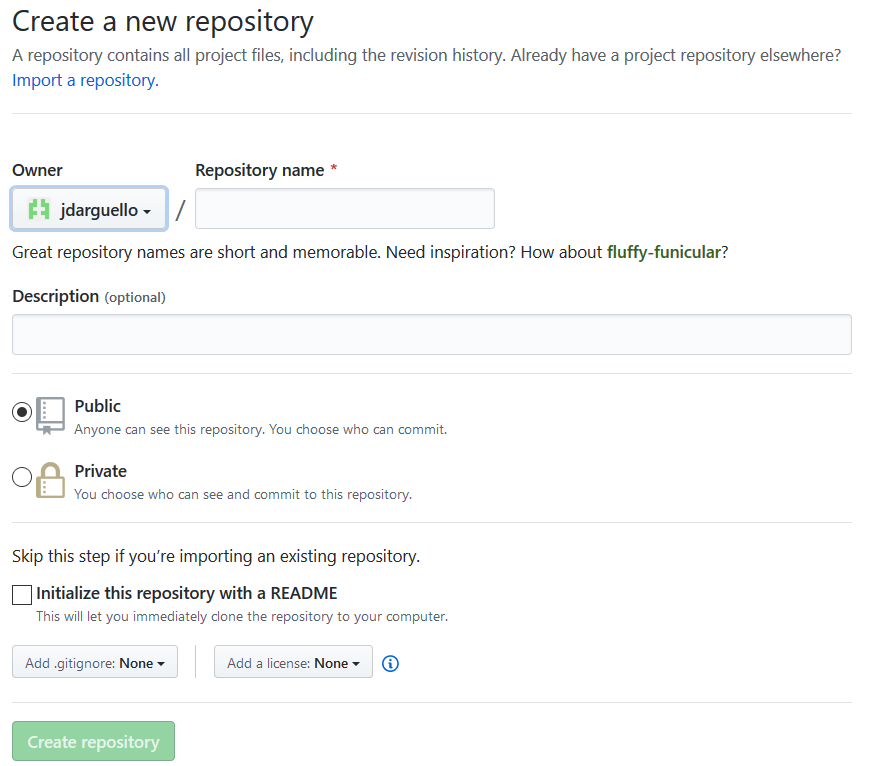
\includegraphics[scale=0.5]{Images/Repositorio.PNG}
\end{figure}

\end{frame}
\begin{frame}[t]{Lectura del código}\vspace{10pt}

El código de programación se ejecuta \textbf{siempre} desde arriba hacia abajo.

\begin{figure}
	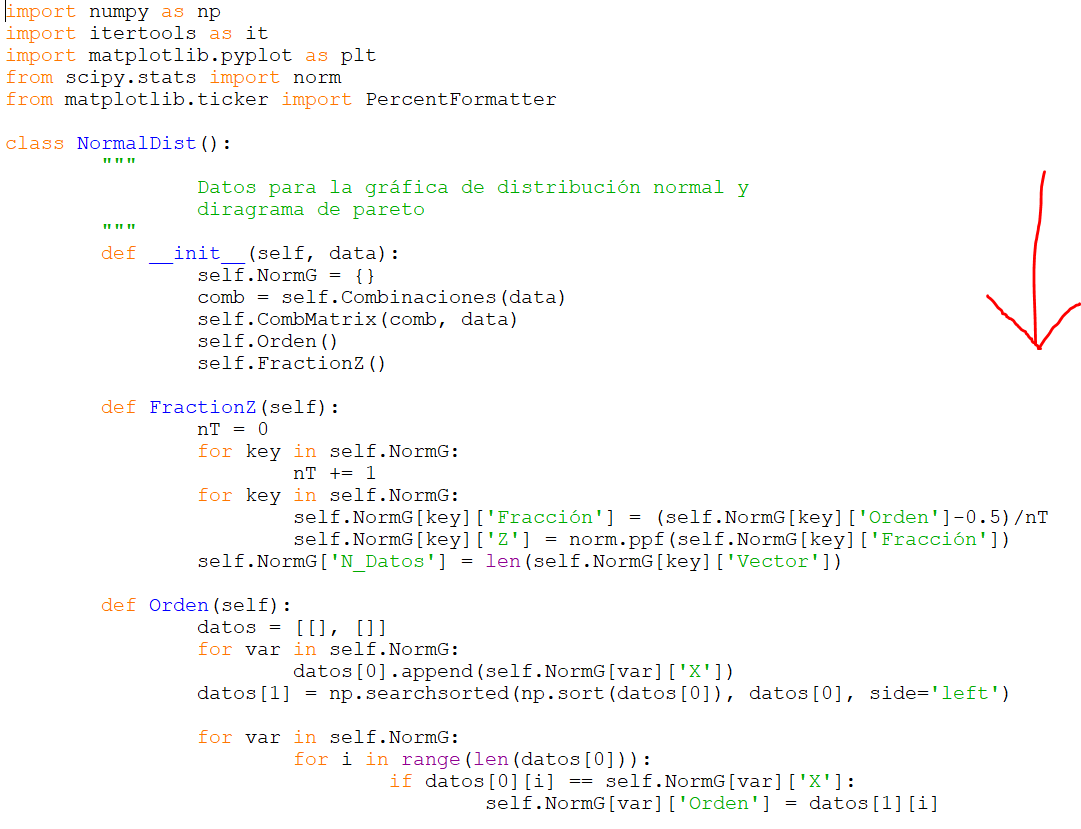
\includegraphics[scale=0.5]{Images/Lectura.PNG}
\end{figure}

\end{frame}
\begin{frame}[t]{Variables en Python}\vspace{10pt}

Empieza \textbf{creando} un ``Script" (archivo de extención .py que contiene el algoritmo de programación). Abre tu editor de texto de preferencia (en mi caso, Sublime Text), y guarda el archivo.

\begin{block}{Guardar código}
	<Nombre del archivo> + '.py'
\end{block}

Crea una variable \textbf{numérica}:

\begin{block}{Crear variable (numérica)}
	x = 2
\end{block}

Para imprimir...
\begin{block}{Imprime!}
	print(x)
\end{block}

\end{frame}
\begin{frame}[t]{Operaciones con Variables}\vspace{10pt}

Ejecuta el algoritmo.
\begin{block}{Pulsa:}
	CTRL + B
\end{block}

Las operaciones básicas...
\begin{block}{Matemática básica...}
	y = (2*(x + 2)**(3*x))/5
\end{block}

Que equivale a...

\begin{equation}
	y = \frac{2 \left(x  + 2 \right)^{3x}}{5}
\end{equation}

\end{frame}
\begin{frame}[fragile]{Archivo de texto}\vspace{10pt}

Podemos leer y escribir archivos de texto con Python (s\'i, tambi\'en podemos crear informes autom\'aticos...). 

\vspace{5pt}

Para \textbf{leer}:

\begin{center}
\begin{lstlisting}
	with open(ruta_archivo, 'r') as file:
		lineas = file.readlines()
\end{lstlisting}
\end{center}

\vspace{5pt}

Para \textbf{escribir}:

\begin{center}
\begin{lstlisting}
	with open(ruta_archivo, 'w+') as file:
		file.write(texto)
\end{lstlisting}
\end{center}


\end{frame}
\begin{frame}[t]{Variables - Listas}\vspace{10pt}

Son vectores \textit{dinámicos}, lo que quiere decir que pueden \textbf{cambiar} sus valores a través del algoritmo de programación.

\vspace{5pt}
Creemos una lista.
\begin{block}{Crear lista}
l = [1, 'Hola', False, 0]
\end{block}

Podemos cambiar un valor.
\begin{block}{¿Terminamos?}
l[1] = 'Chao'
\end{block}

¿De verdad?
\begin{block}{Incrédulo}
l[2] = True
\end{block}

\end{frame}
\begin{frame}[t]{Variables - Tuplas}\vspace{10pt}

Son vectores \textit{estáticos}: \textbf{no} cambian sus componentes durante la ejecución del código.

\vspace{5pt}

Creación de una tupla...
\begin{block}{Tupla}
t = (1, 'Hola', 0)
\end{block}

¿Cambia sus valores?
\begin{block}{No...}
t[1] = 'Chao'
\end{block}

\end{frame}
\begin{frame}[t]{Variables - Diccionario}\vspace{10pt}

Tipo de variable dinámica que \textbf{facilita} la interpretación y el orden del código. Puede contener \textit{cualquier} tipo de variable.

\vspace{5 pt}
Crear un diccionario.
\begin{block}{Crear Diccionario}
dic = \{'Pal': 'Algo', 'Num': 2, 'Bool': True, 'List': [0,'a'], 'Tup': (0,1)\}
\end{block}

Es modificable...
\begin{block}{Modificar Num}
dic['Num'] += 1
\end{block}


\end{frame}
\begin{frame}[t]{Depuración de código}\vspace{10pt}

La depuración consiste en \textbf{probar} el algoritmo lógico.

\vspace{10pt}

\textbf{¿Por qué?}
Fácil: No nos las sabemos todas...

\vspace{10 pt}
Por ejemplo:
\begin{block}{Código que falla...}
z = x/0
\end{block}

\textbf{¿Cómo podemos evitar que falle?}

\begin{itemize}
	\item Sabiendo que ocurre antes del fallo con ``print()".
	\item try - except.
\end{itemize}

\end{frame}
\begin{frame}[fragile]{Depuración de código: try - except}\vspace{10pt}

Lo utilizamos cuando \textbf{no} nos interesa que falle ni el porqué falla. Nos interesa que continúe...

\begin{center}
\begin{lstlisting}
	try:
		z = x/0
	except:
		pass
\end{lstlisting}
\end{center}
\end{frame}
\begin{frame}[t]{Depuración de código - Errores}\vspace{10pt}

Es muy probable que nos encontremos con errores que \textbf{sí} nos interesa solucionar. \textit{¿Qué podemos hacer?}

\vspace{10pt}

Podemos recurrir a {\color{blue}\href{https://stackoverflow.com/}{Stack Overflow}} y buscar problemas \textit{similares} de otros programadores, o \textbf{hacer} nuestras propias preguntas y esperar respuestas.

\end{frame}
\end{document}
